% !TEX root=MemoriaTFG.tex

\chapter{Diseño}\label{diseño}
El correcto diseño de una infraestructura de red es un factor determinante para garantizar la eficiencia, la seguridad y la disponibilidad de los servicios en cualquier entorno,
 y resulta especialmente crítico en instalaciones hospitalarias, donde el funcionamiento continuo de los sistemas de información y de los dispositivos médicos conectados puede 
 tener un impacto directo en la seguridad y atención de los pacientes. Por ello, el diseño debe contemplar no solo la organización topológica de los dispositivos y enlaces, sino
  también la segmentación lógica, las políticas de seguridad y la planificación de los servicios de red necesarios.
\\ \\
En este capítulo se presenta el diseño detallado de la infraestructura de red hospitalaria propuesta, partiendo de los requisitos funcionales, de seguridad y de conectividad 
definidos previamente. El diseño abarca dos niveles: por un lado, la red de interconexión entre los cuatro hospitales simulados, y por otro, el diseño específico y detallado 
de la red de uno de los hospitales, empleando técnicas de segmentación mediante VLANs y subredes diferenciadas para invitados, dispositivos IoMT y servicios internos.
\\ \\
Asimismo, se describen las decisiones adoptadas respecto a la topología física y lógica, la planificación del direccionamiento IP, la definición de las VLANs, la organización 
de los servicios de red, las políticas de seguridad implementadas y la configuración de mecanismos de redundancia y tolerancia a fallos. Todos estos elementos se han planificado
 en base a los criterios de diseño establecidos en capítulos anteriores y conforme a las buenas prácticas recomendadas para entornos sanitarios.
\\ \\
Este capítulo servirá como base para la posterior implementación y simulación de la red en Cisco Packet Tracer, así como para la ejecución de pruebas de conectividad y 
seguridad orientadas a validar su funcionamiento.

\section{Criterios de Diseño}
\label{sec:criterios}
Antes de definir la infraestructura de red, se realizó un análisis de los requisitos funcionales, de seguridad y de conectividad propios de un entorno hospitalario. Este 
análisis, junto con las buenas prácticas en entornos sanitarios, permitió establecer una serie de criterios de diseño, como la segmentación mediante VLANs, el aislamiento 
de subredes críticas como IoMT, la redundancia de enlaces y gateways, y la centralización de servicios en DMZ.
\\ \\
El diseño se divide en dos niveles: una red de interconexión entre cuatro hospitales y un diseño interno detallado de un hospital, dividido en subredes y VLANs según áreas funcionales.
\\  \\
Para la red de interconexión entre hospitales, se optó por simplificar la topología de tal forma que el diseño se enfoque simplemente en la conectividad entre los hospitales, es decir,
se omiten las configuraciones de redundancia (HSRP y EtherChannel) y se simplifica la cantidad de VLANs y subredes, manteniendo la funcionalidad básica de comunicación entre ellos. Esta decisión se tomó 
para no duplicar el esfuerzo de configuración y para centrarse en mejorar las configuraciones de seguridad y conectividad entre los hospitales. 

\section{Topología de Red Propuesta}
En esta sección se presentan las topologías de red propuestas tanto para el Hospital Universitario Son Espases como para la red de interconexión de los cuatro hospitales, que incluye tanto la topología física como la lógica, detallando en cada caso las decisiones adoptadas
y los dispositivos seleccionados para cumplir con los requisitos de conectividad, seguridad y rendimiento.

\subsection{Topología Física Son Espases}
La topología física representa la disposición y conexión física de routers, switches, servidores, dispositivos IoMT y departamentos.
\subsubsection{Routers}
En este diseño, como se muestra en la Figura \ref{fig:Routers}, se han implementado tres routers principales, los cuales están configurados para proporcionar 
redundancia y tolerancia a fallos mediante HSRP (Hot Standby Router Protocol). Estos routers se conectan con:

\begin{itemize}
    \item Red de Invitados.
    \item DMZ Invitados.
    \item DMZ IoMT.
    \item DMZ Interno.
    \item Dos Switches Core.
\end{itemize}

\begin{figure}[H]
    \centering
    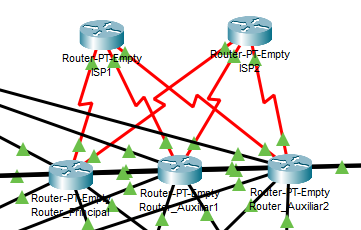
\includegraphics[width=0.4\textwidth]{Imágenes/Routers.png}
    \caption{Redundancia en Routers}
    \label{fig:Routers} 
\end{figure}

Además, estos routers están conectados a dos routers más, que simularían la conexión a Internet (ISP1 y ISP2).

\subsubsection{Red de Invitados}
La red de invitados está diseñada para proporcionar acceso a Internet a los dispositivos de invitados, garantizando que no interfieran con la red interna del hospital. Esta red 
cuenta con dos switches L2 que conectan con dos puntos de acceso inalámbrico (APs) que proporcionan conectividad a los dispositivos móviles de los invitados. La interconexión entre 
el router y la red de invitados se realiza a través de un switch L3, que permite la segmentación y el control del tráfico de red. La Figura \ref{fig:RedInvitados} muestra la topología 
física de la red de invitados.

\begin{figure}[H]
    \centering
    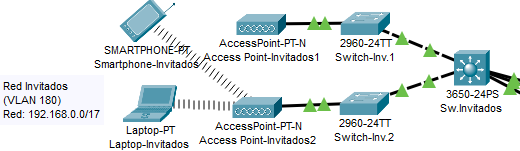
\includegraphics[width=0.6\textwidth]{Imágenes/RedInvitados.png}
    \caption{Topología Física de la Red de Invitados}
    \label{fig:RedInvitados}
\end{figure}

Esta red está muy simplificada, ya que no se han implementado configuraciones de redundancia ni de seguridad avanzadas, centrándose únicamente en la conectividad básica entre los dispositivos 
invitados y el acceso a Internet. Por supuesto, esta red es completamente escalable y se puede ampliar con los dispositivos necesarios para cumplir con futuros requisitos del sistema.

\subsubsection{DMZ Invitados}
La DMZ de invitados está diseñada para dar acceso a Internet a los dispositivos invitados, permitiendo que estos dispositivos tengan una dirección IP única dentro de la red, sin 
interferir con la red interna del hospital. Esta DMZ está conectada a un switch L2 que conecta con los routers, permitiendo la segmentación del tráfico y el control de acceso a los recursos 
internos. La Figura \ref{fig:DMZInvitados} muestra la topología física de la DMZ de invitados.

\begin{figure}[H]
    \centering
    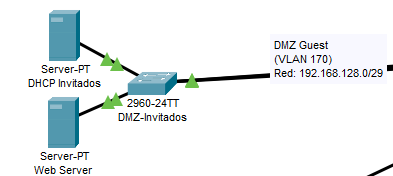
\includegraphics[width=0.5\textwidth]{Imágenes/DMZInvitados.png}
    \caption{Topología Física de la DMZ de Invitados}
    \label{fig:DMZInvitados}
\end{figure}

Como se ha podido ver en la Figura \ref{fig:DMZInvitados}, también se encuentra en esta DMZ el servidor web del hospital, de esta forma los dispsoitivos de Internet que quieuran acceder
a la web del hospital lo harán a través de esta DMZ evitando así que puedan conocer o acceder a la DMZ interna, añadiendo de esta forma una capa extra de seguridad.

\subsubsection{DMZ IoMT}
La DMZ IoMt tiene como finalidad dar direcciones IP dinámicas a los dispositivos IoMT de la red, permitiendo que estos dispositivos puedan tener conectividad con otros dispsoitivos de la red, sin 
que estos servidores DHCP puedan ser detectados o acceddidos por dispositivos externos. Esta DMZ está conectada a un switch L2 que conecta con los routers, permitiendo la segmentación del tráfico 
y el control de acceso a los recursos internos. La Figura \ref{fig:DMZIOMT} muestra la topología física de la DMZ IoMT.

\begin{figure}[H]
    \centering
    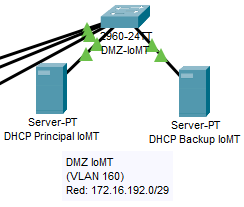
\includegraphics[width=0.35\textwidth]{Imágenes/DMZIOMT.png}
    \caption{Topología Física de la DMZ IoMT}
    \label{fig:DMZIOMT}
\end{figure}

Como se puede apreciar en la Figura \ref{fig:DMZIOMT}, esta DMZ está formada por dos servidores DHCP, uno que está activo y otro en modo reposo, de esta forma se garantiza que si uno de 
los servidores falla, el otro pueda tomar el control y seguir proporcionando direcciones IP a los dispositivos IoMT.

\subsubsection{DMZ Interna}
La DMZ Interna está diseñada para albergar los servidores internos del hospital, como el servidor de correo electrónico, el servidor DNS, el servidor DHCP y el servidor de archivos.
Esta DMZ está conectada a un switch L2 que conecta con los routers, permitiendo la segmentación del tráfico y el control de acceso a los recursos internos. La Figura \ref{fig:DMZInterna} 
muestra la topología física de la DMZ interna.

\begin{figure}[H]
    \centering
    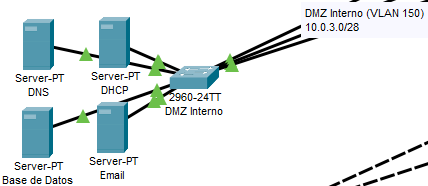
\includegraphics[width=0.5\textwidth]{Imágenes/DMZInterna.png}
    \caption{Topología Física de la DMZ Interna}
    \label{fig:DMZInterna}
\end{figure}

Este servidor de archivos es el encargado de almacenar todos los archivos relevantes que pueden ser compartidos con otros hospitales.

\subsubsection{Red Interna}
La red interna del hospital está diseñada para albergar todos los dispositivos de red y finales del hospital, incluyendo los switches core, los de distribución, los de acceso y los dispositivos finales 
de cada departamento. Dentro de la red interna, primero nos encontramos con los switches core, que conectan con los routers y por tanto dan acceso a Internet y a las DMZ a todos los dispositivos de la red Interna.
Estos switches core están conectados en forma de malla, permitiendo la redundancia y la tolerancia a fallos. La Figura \ref{fig:SwitchesCore} muestra la topología física de la interconexión de los switches core.

\begin{figure}[H]
    \centering
    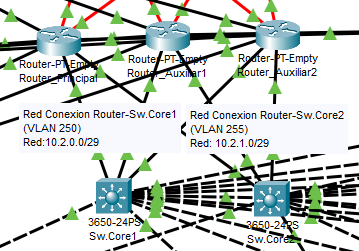
\includegraphics[width=0.5\textwidth]{Imágenes/SwitchesCore.png}
    \caption{Interconexión de Switches Core}
    \label{fig:SwitchesCore}
\end{figure}

Estos switches core están conectados en forma de malla a seis switches de distribución, uno por cada área del hospital (Administración, Servicios Quirúrgicos, Servicios Médicos, Servicios Centrales, Enfermería y Apoyo), 
permitiendo la segmentación del tráfico y el control de acceso a los recursos internos. Además, cada switch de distribución esta conectado a otro dos switches de distribución, 
lo que permite implementar redundancia y tolerancia a fallos. La Figura \ref{fig:SwitchesDistribucion} muestra la topología física de la interconexión de los switches de distribución.

\begin{figure}[H]
    \centering
    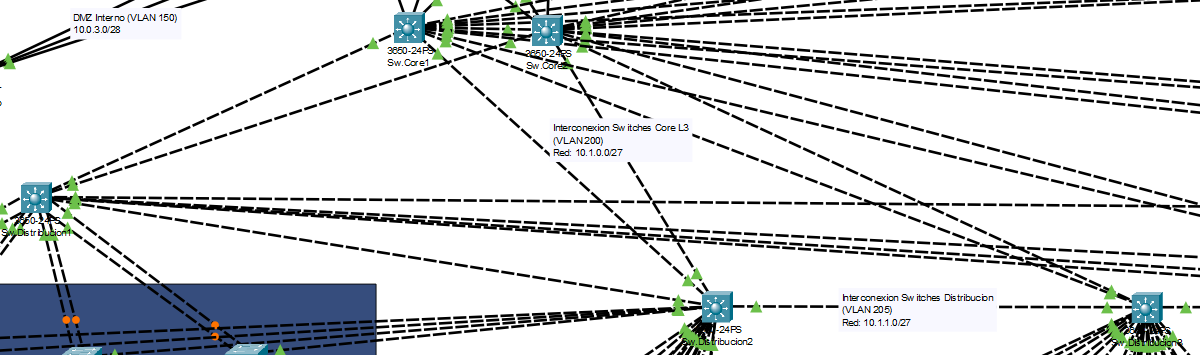
\includegraphics[width=0.7\textwidth]{Imágenes/SwitchesDistribucion.png}
    \caption{Interconexión de Switches de Distribución}
    \label{fig:SwitchesDistribucion}
\end{figure}

Estos switches de distribución están conectados a los switches de acceso, que son los encargados de conectar los dispositivos finales de cada departamento. Cada switch de acceso 
está conectado a dos switches de distribución, permitiendo la redundancia y tolerancia a fallos, además, también tiene un doble enlace con uno de los switches de distribución, 
lo que permite que si uno de los enlaces falla, el otro enlace pueda seguir proporcionando conectividad a los dispositivos finales. La Figura \ref{fig:SwitchesAcceso} muestra la topología física de la interconexión de los switches de acceso.
\begin{figure}[H]
    \centering
    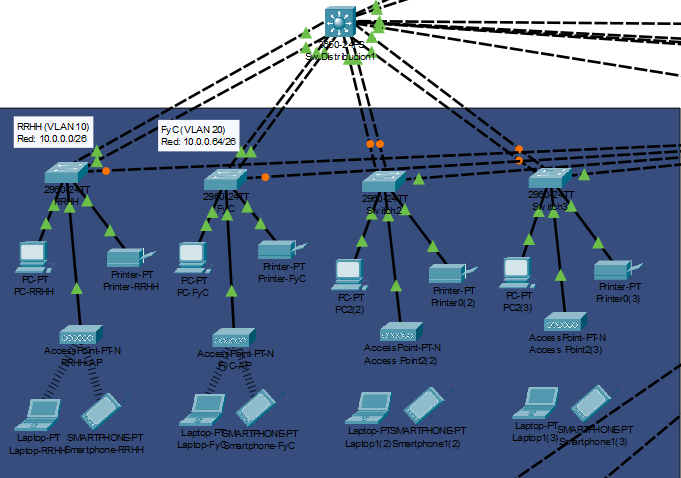
\includegraphics[width=0.6\textwidth]{Imágenes/SwitchesAcceso.png}
    \caption{Interconexión de Switches de Acceso}
    \label{fig:SwitchesAcceso}
\end{figure}

Como se puede ver en la Figura \ref{fig:SwitchesAcceso}, cada departamento esta formado por un PC de escritorio, una impresora y un punto de acceso que da conectividad inalámbrica a un portátil y un smartphone. Esto es así 
a modo de ejemplo, para que se vea que es posible conectar varios dispositivos diferentes y con diferentes conexiones, por supuesto cada departamento es completamente escalable ya que se pueden añadir tantos dispositivos como se necesiten, teneiendo en cuenta que el límite de direcciones IP asignables son 56.

\subsubsection{Red IoMT}
La red IoMT esta conectada directamente a los switches core, de esta forma se consigue que no saturen a los routers con su constante tráfico. En la Figura \ref{fig:IoMT} se muestra la topología física de la red IoMT.
Se puede apreciar claramente que esta dividida en cuatro capas, una por cada planta del hospital, de esta forma podemos distinguir los tipos de dispositivos IoMT según la planta en la que se encuentren. 
Cada capa está formada por un switch L3 que conecta con tres puntos de acceso, lo que permite que haya cobertura inalámbrica a lo largo de cada planta, y además permite que si los dispositivos IoMT se desplazan, puedan coenctarse a otro punto de acceso bajo el mismo SSID.
 
\begin{figure}[H]
    \centering
    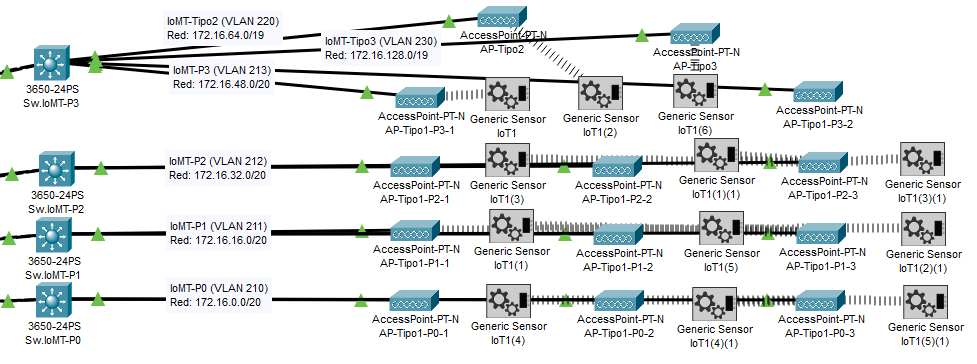
\includegraphics[width=0.65\textwidth]{Imágenes/IoMT.png}
    \caption{Topología Física de la Red de Dispositivos IoMT}
    \label{fig:IoMT}
\end{figure}

\subsubsection{Disposición Física}
\label{subsubsec:dispsoicion}
La Figura \ref{fig:disposicion} muestra una imagen en tres dimensiones de la disposición de los dispositivos de red y diferentes departamentos del hospital, de esta forma se puede apreciar 
de forma mas clara la disposición física de los diferentes elementos de la red. La ubicación de algunos departamentos se ha extraído de un vídeo de Youtube publicado por el Govern de les Illes Balears \cite{SonEspases}.
\begin{figure}[H]
    \centering
    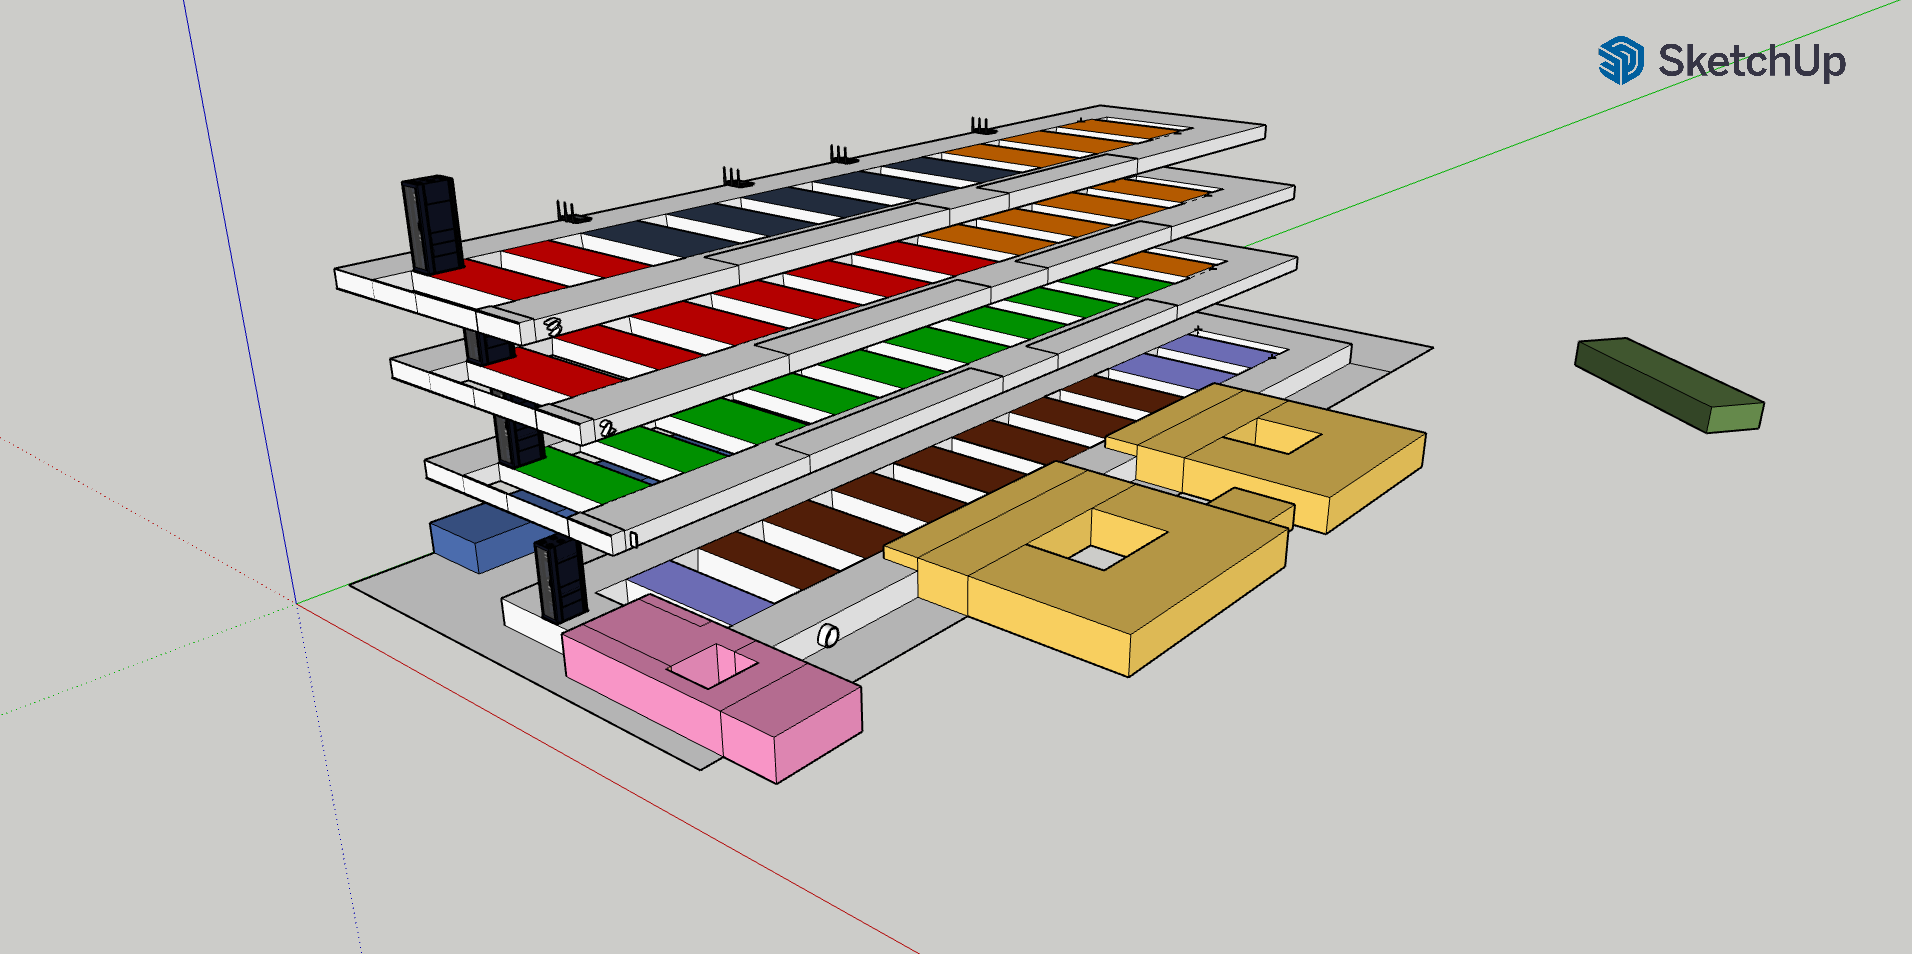
\includegraphics[width=0.6\textwidth]{Imágenes/Plano Son Espases.png}
    \caption{Disposición Física Elementos de Red del Hospital Son Espases}
    \label{fig:disposicion}
\end{figure}
Además, las grandes áreas y departamentos del Hospital de Son Espases se han extraído de sitios web oficiales del Govern de les Illes Balears, como el portal de Gerencia del Hospital Universitario de Son Espases 
\cite{GerenciaSonEspases} o el documento oficial de la plantilla del Hospital Universitario de Son Espases \cite{PlantillaSonEspases}.

\subsection{Topología Lógica Son Espases}

La topología lógica define la organización del tráfico y las relaciones entre las distintas VLANs, subredes y servicios.
\\ \\
En este diseño, se ha definido una VLAN por cada departamento del hospital, así como VLANs específicas para servicios críticos como IoMT, red de invitados e interconexiones entre dispositivos de red. También se han definido tres grandes subredes:
\begin{itemize}
    \item \textbf{Subred Interna:} Esta subred alberga las VLANs de los departamentos y servicios internos del hospital, garantizando la comunicación entre ellos y el acceso a los recursos compartidos.
    \item \textbf{Subred IoMT:} Esta subred está dedicada a los dispositivos IoMT, garantizando su aislamiento y seguridad, así como la monitorización de su tráfico.
    \item \textbf{Subred de Invitados:} Esta subred permite el acceso a Internet y a servicios básicos para los dispositivos de invitados, garantizando que no interfieran con la red interna del hospital.
\end{itemize}

Además de esas subredes, también se han definido algunas VLANs específicas para la interconexión entre dispositivos de red, como los routers y switches core, así como para la DMZ interna y la DMZ IoMT.
\\ \\
La subred IoMT esta formada por una VLAN por cada planta, exceptuando la última planta, en la que hay tres VLANs distintas, esto es debido a que en esa planta es donde se encuentra la UCI, y por tanto los dispositivos IoMT de tipo 2 y 3.
Por ese motivo, hay una VLAN para cada tipo de dispositivo IoMT en la planta 3, con esto se consigue una segmentación de red robusta y además se mejora la seguridad ya que se pueden implementar medidas de control de tráfico para filtrar según el tipo de dispositivo IoMT al que estén accediendo.
\\ \\
{\small \textbf{Nota:} \textit{Para recordar los tipos de dispositivos IoMT que hay, ver la sección \ref{subsec: TiposIoMT}}}


\subsection{Topología Física de la Red de Interconexión entre Hospitales}
Este diseño es el mismo para los cuatro hospitales, permitiendo así que todos dispongan de los mismos recursos, aunque individualmente cada uno tenga sus propios departamentos.
En este diseño, el núcleo de la red es la interconexión de los cuatro hospitales, esta se lleva a cabo mediante enlaces directos entre cada router de cada hospital, en la Figura \ref{fig:InterconexionHospitales}
se muestra la topología física de los routers de interconexión entre hospitales.

\begin{figure}[H]
    \centering
    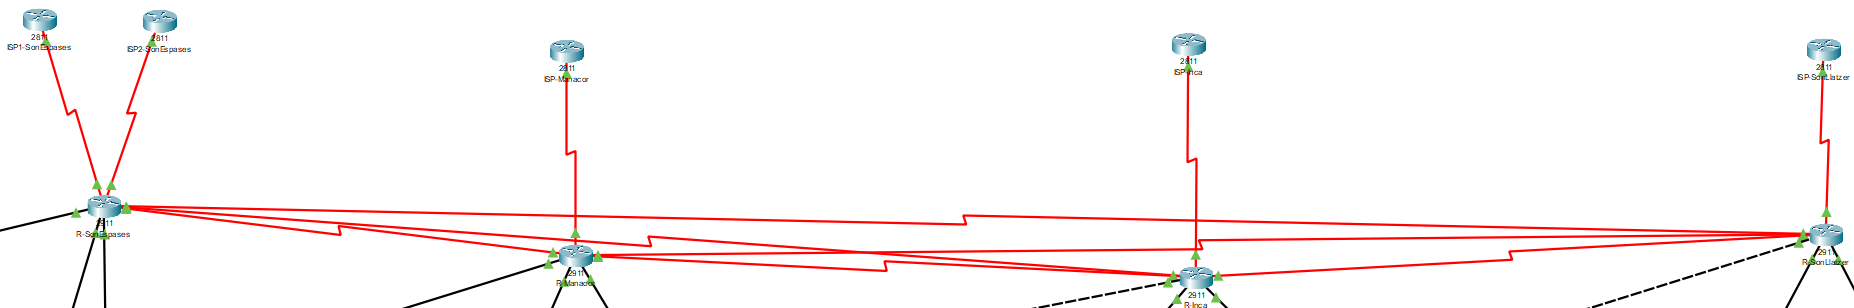
\includegraphics[width=0.6\textwidth]{Imágenes/InterconexionHospitales.png}
    \caption{Topología Física de la Interconexión entre Hospitales}
    \label{fig:InterconexionHospitales}
\end{figure}

Como se puede apreciar en la Figura \ref{fig:InterconexionHospitales}, cada hospital tiene un único router conectado a otro router, simulando así la conexión a Internet, excepto en el caso del Hospital de Son Espases, que 
tiene dos ISPs distintos, ya que al ser el hospital principal, se ha decidido que tenga dos conexiones a Internet para garantizar la redundancia y la tolerancia a fallos.
\\ \\
Además, cada router de cada hospital está conectado a dos switches core (L3), que son los que dan conectividad con el router a todos los dispositivos de la red interna, en la Figura 
\ref{fig:InterconexionRouHospitales} se muestra la topología física de la interconexión entre el router y los switches core. 

\begin{figure}[H]
    \centering
    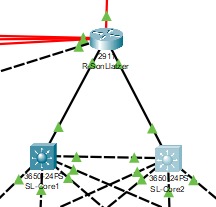
\includegraphics[width=0.3\textwidth]{Imágenes/Router-Sw.Core.png}
    \caption{Topología Física de la Interconexión entre el Router y los Switches Core en Hospitales}
    \label{fig:InterconexionRouHospitales}
\end{figure}

Los dos switches core también estan conectados en forma de malla con 4 switches de distribución, uno por cada area del hospital (Administración, Áreas Médicas, Enfermeria, Área de Apoyo). 
Con el fin de conseguir redundancia y tolerancia a fallos, estos switches de distribución se interconectan entre ellos dos a dos. En la Figura \ref{fig:InterconexionSwHospitales} se muestra la topología de interconexión entre los switches core y los switches de distribución.

\begin{figure}[H]
    \centering
    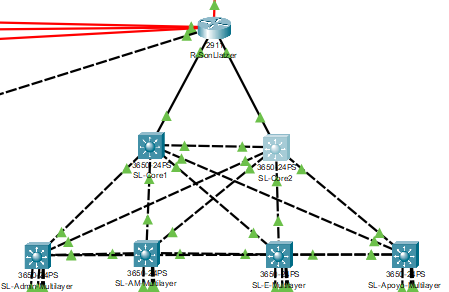
\includegraphics[width=0.5\textwidth]{Imágenes/Switches.png}
    \caption{Topología Física de la Interconexión entre los Switches L3 en Hospitales}
    \label{fig:InterconexionSwHospitales}
\end{figure}

A su vez, los switches de distribución conectan con los switches de acceso, los cuales dan conectividad a los dispositivos finales. En la Figura \ref{fig:CLustersHospitales} se aprecia como, con fines de 
ahorrar espacio y tener la red mas ordenada, los switches de distribución se conectan con un cluster, el cual contiene los switches de acceso y por tanto las VLANs de cada departamento, separadas 
según las principales áreas del hospital.

\begin{figure}[H]
    \centering
    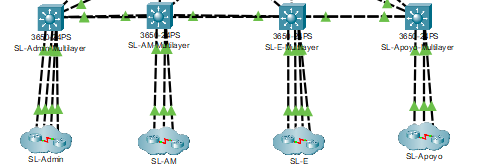
\includegraphics[width=0.55\textwidth]{Imágenes/Clusters.png}
    \caption{Topología Física de la Interconexión con Clusters en Hospitales}
    \label{fig:CLustersHospitales}
\end{figure}

En la Figura \ref{fig:CLustersDentroHospitales} se aprecian las subredes que hay dentro de los clusters, en este caso es la subred del area de adminsitración, la cual se compone por el departamento de Recursos Humanos, Finnazas y Contabilidad, Tecnologías de la Información y Servicios Generales.
\begin{figure}[H]
    \centering
    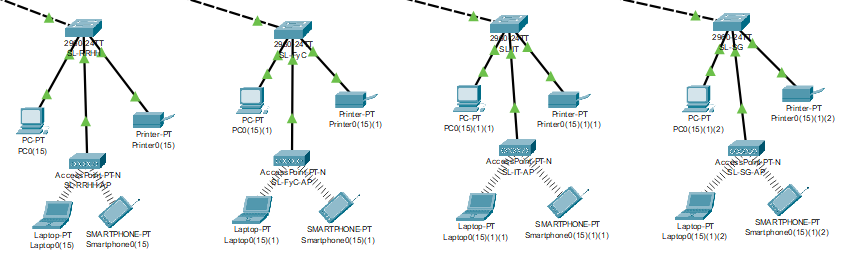
\includegraphics[width=0.5\textwidth]{Imágenes/CLusterdentro.png}
    \caption{Topología Física de la Interconexión con Clusters en Hospitales}
    \label{fig:CLustersDentroHospitales}
\end{figure}


\subsection{Topología Lógica de la Red de Interconexión entre Hospitales}
En este diseño, se ha definido una VLAN por cada departamento del hospital, además de las VLANs de interconexión entre switches y routers. Además, se han definido cuatro grandes subredes:
\begin{itemize}
    \item \textbf{Subred Son Espases:} Esta subred alberga las VLANs de los departamentos y servicios internos del Hospital Son Espases, garantizando la comunicación entre ellos y el acceso a los recursos compartidos.
    \item \textbf{Subred Manacor:} Esta subred alberga las VLANs de los departamentos y servicios internos del Hospital de Manacor, garantizando la comunicación entre ellos y el acceso a los recursos compartidos.
    \item \textbf{Subred Inca:} vEsta subred alberga las VLANs de los departamentos y servicios internos del Hospital Comarcal de Inca, garantizando la comunicación entre ellos y el acceso a los recursos compartidos.
    \item \textbf{Subred Son Llàtzer:} Esta subred alberga las VLANs de los departamentos y servicios internos del Hospital Son Llàtzer, garantizando la comunicación entre ellos y el acceso a los recursos compartidos.
\end{itemize}
Cada hospital tiene su propia DMZ, donde alberga los servidores necesarios para dar los servicios al hospital y además cuenta con un servidor de archivos, que almacena información relevante del hospital, con el fin de que sea accesible por dispositivos autorizados de otros hospitales.

\subsection{Descripción de Dispositivos Utilizados}

En ambos diseños se han utilizado los siguientes dispositivos:
\begin{itemize}
    \item \textbf{Routers:} Se ha utilizado el modelo \textit{Router-PT-Empty}, ya que permite añadir la cantidad de interfaces tanto GigabitEthernet como Serial necesarias para realizar 
    las conexiones.
    \item \textbf{Switches L2:} Se ha utilizado el modelo \textit{2960 IOS15}, ya que es el modelo mas moderno que ofrece la herramienta Cisco Packet Tracer.
    \item \textbf{Switches L3:} Se ha utilizado el modelo \textit{3650-24PS}, ya que es el modelo mas moderno que ofrece la herramienta Cisco Packet Tracer.
    \item \textbf{Puntos de Acceso Inalámbrico:} Se ha utilizado el modelo \textit{AccessPoint-PT-N}, ya que es el modelo mas potente de los ofrecidos por la herramienta Cisco Packet Tracer.
    \item \textbf{Dispositivos Finales:} 
    \begin{itemize}
        \item \textbf{Portátiles:} \textit{Laptop-PT}
        \item \textbf{PCs de Escritorio:} \textit{PC-PT}
        \item \textbf{Dispositivos Móviles:} \textit{Smartphone-PT}
        \item \textbf{Impresoras:} \textit{Printer-PT}
        \item \textbf{Dispositivos IoMT:} \textit{Generic Sensor}
        \item \textbf{Servidores:} \textit{Server-PT}
    \end{itemize}
\end{itemize}

El cableado utilizado en toda la red es de tipo \textit{Cobre}, mientras que las conexiones entre los routers y los ISPs se realizan mediante cableado de tipo \textit{Serial}.

\section{VLANs y Segmentación de Red}
Uno de los elementos esenciales para garantizar la seguridad, la eficiencia y la organización de una infraestructura de red hospitalaria es la correcta segmentación del 
tráfico mediante el uso de Virtual LANs (VLANs). En este proyecto se ha diseñado una segmentación lógica basada en la estructura funcional de los hospitales, asignando una 
VLAN diferente a cada área o departamento, y separando además las subredes críticas como la de invitados y la de dispositivos IoMT.
\\ \\
Este enfoque permite aislar el tráfico de cada grupo de dispositivos, reducir la propagación de posibles ataques, evitar la congestión de tráfico y facilitar la aplicación de 
políticas de seguridad específicas entre diferentes segmentos de la red.

\subsection{Definición de VLANs por Departamento}
\label{subsec:VLANs}
Cada hospital se ha organizado internamente mediante VLANs asignadas a los diferentes departamentos y servicios. En el caso de la red de Son Espases, se han definido y configurado 
las siguientes VLANs: 
\begin{itemize}
    \item \textbf{VLAN 10:} RRHH (Recursos Humanos)
    \item \textbf{VLAN 20:} FyC (Finanzas y Contabilidad)
    \item \textbf{VLAN 30:} Oftalmologia
    \item \textbf{VLAN 40:} Urologia 
    \item \textbf{VLAN 50:} Cardiologia 
    \item \textbf{VLAN 60:} Dermatologia 
    \item \textbf{VLAN 70:} Radiologia 
    \item \textbf{VLAN 80:} Inmunologia 
    \item \textbf{VLAN 90:} Admision
    \item \textbf{VLAN 100:} UCI (Unidad de Cuidados Intensivos)
    \item \textbf{VLAN 110:} Atencion paciente 
    \item \textbf{VLAN 120:} Asesoria Jurídica
    \item \textbf{VLAN 150:} DMZ Interno
    \item \textbf{VLAN 160:} DMZ IoMT
    \item \textbf{VLAN 170:} DMZ Invitados
    \item \textbf{VLAN 180:} Red Invitados
    \item \textbf{VLAN 190:} Interconexión Router-Sw.Invitados
    \item \textbf{VLAN 200:} Interconexión Switches Distribución - Switches Core
    \item \textbf{VLAN 205:} Interconexión Switches Distribución
    \item \textbf{VLAN 210:} Red IoMT Tipo 1 Planta 0
    \item \textbf{VLAN 211:} Red IoMT Tipo 1 Planta 1
    \item \textbf{VLAN 212:} Red IoMT Tipo 1 Planta 2
    \item \textbf{VLAN 213:} Red IoMT Tipo 1 Planta 3
    \item \textbf{VLAN 220:} Red IoMT Tipo 2 Planta 3
    \item \textbf{VLAN 230:} Red IoMT Tipo 3 Planta 3
    \item \textbf{VLAN 250:} Interconexión Routers - Switch Core 1
    \item \textbf{VLAN 255:} Interconexión Routers - Switch Core 2
\end{itemize}

En el caso de la red de interconexión entre hospitales, se han definido las siguientes VLANs para el hospital de Son Espases:
\begin{itemize}
    \item \textbf{VLAN 10:} RRHH (Recursos Humanos)
    \item \textbf{VLAN 20:} FyC (Finanzas y Contabilidad)
    \item \textbf{VLAN 30:} IT (Tecnologías de la Información)
    \item \textbf{VLAN 40:} SG (Servicios Generales)
    \item \textbf{VLAN 50:} SQ (Servicios Quirúrgicos)
    \item \textbf{VLAN 60:} SM (Servicios Médicos)
    \item \textbf{VLAN 70:} SC (Servicios Centrales)
    \item \textbf{VLAN 80:} UA (Unidad de Admisión)
    \item \textbf{VLAN 90:} UCI (Unidad de Cuidados Intensivos)
    \item \textbf{VLAN 100:} SU (Servicio de Urgencias)
    \item \textbf{VLAN 110:} CE (Consultas Externas)
    \item \textbf{VLAN 120:} AP (Atención al Paciente)
    \item \textbf{VLAN 130:} AJ (Asesoria Jurídica)
    \item \textbf{VLAN 140:} DeI (Docencia e Investigación)
    \item \textbf{VLAN 180:} DMZ Son Espases
    \item \textbf{VLAN 200:} Interconexión Switches Distribución - Switches Core
\end{itemize}

Para la red del Hospital de Manacor, se han definido las siguientes VLANs:
\begin{itemize}
    \item \textbf{VLAN 210:} RRHH (Recursos Humanos)
    \item \textbf{VLAN 220:} FyC (Finanzas y Contabilidad)
    \item \textbf{VLAN 230:} IT (Tecnologías de la Información)
    \item \textbf{VLAN 240:} SG (Servicios Generales)
    \item \textbf{VLAN 250:} SQ (Servicios Quirúrgicos)
    \item \textbf{VLAN 260:} SM (Servicios Médicos)
    \item \textbf{VLAN 270:} SC (Servicios Centrales)
    \item \textbf{VLAN 280:} UA (Unidad de Admisión)
    \item \textbf{VLAN 290:} SU (Servicio de Urgencias)
    \item \textbf{VLAN 300:} CE (Consultas Externas)
    \item \textbf{VLAN 310:} AP (Atención al Paciente)
    \item \textbf{VLAN 320:} AJ (Asesoria Jurídica)
    \item \textbf{VLAN 380:} Interconexión Switches Distribución - Switches Core
    \item \textbf{VLAN 400:} DMZ Manacor
\end{itemize}

Para la red del Hospital Comarcal de Inca, se han definido las siguientes VLANs:
\begin{itemize}
    \item \textbf{VLAN 410:} RRHH (Recursos Humanos)
    \item \textbf{VLAN 420:} FyC (Finanzas y Contabilidad)
    \item \textbf{VLAN 430:} IT (Tecnologías de la Información)
    \item \textbf{VLAN 440:} SG (Servicios Generales)
    \item \textbf{VLAN 450:} SQ (Servicios Quirúrgicos)
    \item \textbf{VLAN 460:} SM (Servicios Médicos)
    \item \textbf{VLAN 470:} SC (Servicios Centrales)
    \item \textbf{VLAN 480:} UA (Unidad de Admisión)
    \item \textbf{VLAN 490:} SU (Servicio de Urgencias)
    \item \textbf{VLAN 500:} CE (Consultas Externas)
    \item \textbf{VLAN 510:} UCI (Unidad de Cuidados Intensivos)
    \item \textbf{VLAN 520:} AP (Atención al Paciente)
    \item \textbf{VLAN 530:} AJ (Asesoria Jurídica)
    \item \textbf{VLAN 580:} Interconexión Switches Distribución - Switches Core
    \item \textbf{VLAN 600:} DMZ Inca
\end{itemize}

Para la red del Hospital Son Llàtzer, se han definido las siguientes VLANs:
\begin{itemize}
    \item \textbf{VLAN 610:} RRHH (Recursos Humanos)
    \item \textbf{VLAN 620:} FyC (Finanzas y Contabilidad)
    \item \textbf{VLAN 630:} IT (Tecnologías de la Información)
    \item \textbf{VLAN 640:} SG (Servicios Generales)
    \item \textbf{VLAN 650:} SQ (Servicios Quirúrgicos)
    \item \textbf{VLAN 660:} SM (Servicios Médicos)
    \item \textbf{VLAN 670:} SC (Servicios Centrales)
    \item \textbf{VLAN 680:} UA (Unidad de Admisión)
    \item \textbf{VLAN 690:} SU (Servicio de Urgencias)
    \item \textbf{VLAN 700:} CE (Consultas Externas)
    \item \textbf{VLAN 710:} UCI (Unidad de Cuidados Intensivos)
    \item \textbf{VLAN 720:} AP (Atención al Paciente)
    \item \textbf{VLAN 730:} AJ (Asesoria Jurídica)
    \item \textbf{VLAN 740:} DeI (Docencia e Investigación)
    \item \textbf{VLAN 780:} Interconexión Switches Distribución - Switches Core
    \item \textbf{VLAN 800:} DMZ Son Llàtzer
\end{itemize}

En el caso de la red de Son Espases, se ha optado por configurar solamente los departamentos mostrados anteriormente, realmente hay muchos mas departamentos \cite{GerenciaSonEspases}, pero con el objetivo
de no duplicar esfuerzos en la configuración de dispositivos irrelevantes, se ha optado por no configurar el resto de departamentos.
\\ \\
En el caso de la red de interconexión entre hospitales, se ha optado por configurar todos los departamentos de los hospitales, con el fin de probar la conectividad desde cualquier area o 
departamento de un hospital a cualquier area o departamento de otro hospital.

\subsection{Configuración de Troncales y Acceso a VLANs}
Para garantizar el correcto funcionamiento de las VLANs y la segmentación del tráfico, es necesario configurar los puertos de los switches siguiendo el siguiente criterio:
\begin{itemize}
    \item \textbf{Switches de Acceso (L2)} 
    \begin{itemize}
        \item \textbf{FastEthernet:} Son los puertos que conectan con los dispositivos finales (PCs, impresoras, servidores, etc.), se configuran en modo acceso, asignándolos a la VLAN correspondiente 
        del departamento o servicio al que pertenecen.
        \item \textbf{GigabitEthernet:} Son los puertos que conectan con los switches de distribución o routers (en el caso de los switches del DMZ), se configuran en modo troncal, permitiendo el tráfico de la VLAN definida en ese departamento o servicio.
    \end{itemize}
    \item \textbf{Switches de Distribución (L3):} Todos los puertos deben estar configurados en modo troncal, permitiendo el tráfico de todas las VLANs necesarias.
    \item \textbf{Switches Core (L3):} Todos los puertos conectados a los switches de distribución deben estar configurados en modo troncal, permitiendo el tráfico de todas las VLANs necesarias. Los puertos que conectan con los routers 
    tienen dirección IP estática y por lo tanto no se configura el switchport en modo troncal.
\end{itemize}

\section{Direccionamiento IP y Subnetting}\label{sec:direccionamiento}
Un correcto esquema de direccionamiento IP es esencial para garantizar la organización, la escalabilidad y la seguridad de cualquier infraestructura de red. En entornos 
hospitalarios, donde coexisten diferentes tipos de dispositivos y servicios con requisitos de conectividad y seguridad distintos, la planificación del direccionamiento 
cobra especial relevancia.
\\ \\
Para este proyecto se ha diseñado un esquema jerárquico y estructurado, basado en subredes independientes para cada entorno funcional y departamental, facilitando la 
segmentación del tráfico, la implementación de políticas de seguridad y la gestión de direcciones IP.

\subsection{Criterios de Diseño de Direccionamiento}
El esquema de direccionamiento se ha planificado atendiendo a los siguientes criterios:
\begin{itemize}
    \item Separación de subredes por tipo de servicio: red de invitados, red IoMT y red interna hospitalaria.
    \item Uso de rangos de direcciones IP privadas (192.168.0.0/16, 172.16.0.0/12 y 10.0.0.0/8), según las recomendaciones de la RFC 1918.
    \item Evitar solapamientos entre subredes y facilitar su integración en redes hospitalarias de mayor escala.
    \item Facilitar la implementación de ACLs y políticas de seguridad basadas en rangos de IP.
    \item Garantizar escalabilidad para añadir nuevos dispositivos, departamentos o servicios en el futuro.
\end{itemize}

\subsection{Planificación de Subredes}
En el diseño de la red del Hospital de Son Espases, se han definido tres grandes subredes principales:
\begin{itemize}
    \item \textbf{Red Invitados:} 192.168.0.0/16
    \item \textbf{Red Interna:} 10.0.0.0/8
    \item \textbf{Red IoMT:} 172.16.0.0/12
\end{itemize}
Aparte de estas redes también están las subredes de interconexión entre switches y routers. En la tabla \ref{tab:subnettingSonEspases} podemos ver el subnetting completo de la red del Hospital de 
Son Espases. En la tabla se puede apreciar que hay 5 columnas, a continuación se muestra una breve descripción de cada una:
\begin{enumerate}
    \item \textbf{Departamento:} Es el nombre del área o servicio funcional al que pertenece esa subred o VLAN. Por ejemplo: UCI.
    \item \textbf{Network Address:} Es la dirección de red que identifica a toda la subred. Es la primera dirección del bloque de direcciones IP asignadas a esa subred 
    y no puede asignarse a ningún dispositivo. Sirve para que los routers y switches reconozcan la red en su tabla de enrutamiento. Por ejemplo: 192.168.0.0.
    \item \textbf{Máscara de Subred:} Es el valor que determina cuántos bits se utilizan para identificar la parte de red y cuántos para los hosts dentro de esa subred. 
    Se expresa en notación decimal, por ejemplo 255.255.255.0.
    \item \textbf{Rango de Direcciones Host:} Indica las direcciones IP que se pueden asignar a dispositivos dentro de esa subred. Es el intervalo de direcciones 
    comprendido entre la primera dirección válida y la dirección anterior a la de broadcast. Por ejemplo, 192.168.0.1.
    \item \textbf{Dirección Broadcast:} Es la última dirección de cada subred. Se utiliza para enviar mensajes simultáneos a todos los dispositivos de esa subred. No se 
    puede asignar a ningún dispositivo. Por ejemplo, 192.168.0.255 para la subred 192.168.0.0/24.
\end{enumerate}

{\small \textbf{Nota: }\textit{Las VLANs correspondientes a cada subred están definidas en la sección \ref{subsec:VLANs}}}

\subsubsection{Subnetting Son Espases}
En la Tabla \ref{tab:subnettingSonEspases} se muestra en detalle el subnetting realizado en la red interna del Hospital Son Espases.

\renewcommand{\arraystretch}{1.3}
\begin{table}[H]
    \centering
    \scriptsize
    \begin{tabular}{|l|c|c|c|c|}
        \hline
        \textbf{Departamento} & \textbf{Network Address} & \textbf{Máscara de Subred} & \textbf{Direcciones Host} & \textbf{Dirección Broadcast} \\
        \hline
        Recursos Humanos & 10.0.0.0 & 255.255.255.192 & 10.0.0.1 - 10.0.0.62 & 10.0.0.63 \\
        \hline
        Contabilidad & 10.0.0.64 & 255.255.255.192 & 10.0.0.65 - 10.0.0.126 & 10.0.0.127 \\
        \hline
        Oftalmología & 10.0.0.128 & 255.255.255.192 & 10.0.0.129 - 10.0.0.190 & 10.0.0.191 \\
        \hline
        Urología & 10.0.0.192 & 255.255.255.192 & 10.0.0.193 - 10.0.0.254 & 10.0.0.255 \\
        \hline
        Cardiología & 10.0.1.0 & 255.255.255.192 & 10.0.1.1 - 10.0.1.62 & 10.0.1.63 \\
        \hline
        Dermatología & 10.0.1.64 & 255.255.255.192 & 10.0.1.65 - 10.0.1.126 & 10.0.1.127 \\
        \hline
        Radiología & 10.0.1.128 & 255.255.255.192 & 10.0.1.129 - 10.0.1.190 & 10.0.1.191 \\
        \hline
        Inmunología & 10.0.1.192 & 255.255.255.192 & 10.0.1.193 - 10.0.1.254 & 10.0.1.255 \\
        \hline
        Unidad Admisión & 10.0.2.0 & 255.255.255.192 & 10.0.2.1 - 10.0.2.62 & 10.0.2.63 \\
        \hline
        UCI & 10.0.2.64 & 255.255.255.192 & 10.0.0.65 - 10.0.2.126 & 10.0.2.127 \\
        \hline
        Atención Paciente & 10.0.2.128 & 255.255.255.192 & 10.0.2.129 - 10.0.2.190 & 10.0.2.191 \\
        \hline
        Asesoría Jurídica & 10.0.2.192 & 255.255.255.192 & 10.0.2.193 - 10.0.2.254 & 10.0.2.255 \\
        \hline
        DMZ & 10.0.3.0 & 255.255.255.240 & 10.0.3.1 - 10.0.3.14 & 10.0.3.15 \\
        \hline
    \end{tabular}
    \caption{Subnetting Red Interna Son Espases}
    \label{tab:subnettingSonEspases}
\end{table}

En las Tablas \ref{tab:InterconexionCoreSE}, \ref{tab:InterconexionDistrSE}, \ref{tab:InterconexionCore1-RouterSE}, \ref{tab:InterconexionCore2-RouterSE} y \ref{tab:InterconexionRouter-ISPSE},
se pueden apreciar el subnetting de las interconexiones anteriormente mencionadas.
\renewcommand{\arraystretch}{1.5}
\begin{table}[H]
    \centering
    \scriptsize
    \begin{tabular}{|l|c|}
        \hline
        \textbf{Dispositivos} & \textbf{Dirección IP} \\
        \hline
        Switch Distribución 1 (Administración) & 10.1.0.1 \\
        \hline
        Switch Distribución 2 (Serv. Quirúrgicos) & 10.1.0.2 \\
        \hline
        Switch Distribución 3 (Serv. Médicos) & 10.1.0.3 \\
        \hline
        Switch Distribución 4 (Serv. Centrales) & 10.1.0.4 \\
        \hline
        Switch Distribución 5 (Enfermería) & 10.1.0.5 \\
        \hline
        Switch Distribución 6 (Apoyo) & 10.1.0.6 \\
        \hline
        Switch Core 1 & 10.1.0.7 \\
        \hline
        Switch Core 2 & 10.1.0.8 \\
        \hline
        Switch IoMT-P0 & 10.1.0.9 \\
        \hline
        Switch IoMT-P1 & 10.1.0.10 \\
        \hline
        Switch IoMT-P2 & 10.1.0.11 \\
        \hline
        Switch IoMT-P3 & 10.1.0.12 \\
        \hline
    \end{tabular}
    \caption{Subnetting Red Interconexión Switches Distribución - Switches Core}
    \label{tab:InterconexionCoreSE}
\end{table}

\begin{table}[H]
    \centering
    \scriptsize
    \begin{tabular}{|l|c|}
        \hline
        \textbf{Dispositivo} & \textbf{Dirección IP} \\
        \hline
        Switch Distribución 1 (Administración) & 10.1.1.1 \\
        \hline
        Switch Distribución 2 (Serv. Quirúrgicos) & 10.1.1.2 \\
        \hline
        Switch Distribución 3 (Serv. Médicos) & 10.1.1.3 \\
        \hline
        Switch Distribución 4 (Serv. Centrales) & 10.1.1.4 \\
        \hline
        Switch Distribución 5 (Enfermería) & 10.1.1.5 \\
        \hline
        Switch Distribución 6 (Apoyo) & 10.1.1.6 \\
        \hline
    \end{tabular}
    \caption{Subnetting Red Interconexión Switches Distribuidores}
    \label{tab:InterconexionDistrSE}
\end{table}

\begin{table}[H]
    \centering
    \scriptsize
    \begin{tabular}{|l|c|}
        \hline
        \textbf{Dispositivo} & \textbf{Dirección IP} \\
        \hline
        IP Virtual & 10.2.0.1 \\
        \hline
        Router Principal & 10.2.0.2 \\
        \hline
        Router Auxiliar 1 & 10.2.0.3 \\
        \hline
        Router Auxiliar 2 & 10.2.0.4 \\
        \hline
        Switch Core 1 & 10.2.0.5 \\
        \hline
    \end{tabular}
    \caption{Subnetting Red Interconexión Switch Core 1 - Routers}
    \label{tab:InterconexionCore1-RouterSE}
\end{table}

\begin{table}[H]
    \centering
    \scriptsize
    \begin{tabular}{|l|c|}
        \hline
        \textbf{Dispositivo} & \textbf{Dirección IP} \\
        \hline
        IP Virtual & 10.2.1.1 \\
        \hline
        Router Principal & 10.2.1.2 \\
        \hline
        Router Auxiliar 1 & 10.2.1.3 \\
        \hline
        Router Auxiliar 2 & 10.2.1.4 \\
        \hline
        Switch Core 1 & 10.2.1.5 \\
        \hline
    \end{tabular}
    \caption{Subnetting Red Interconexión Switch Core 2 - Routers}
    \label{tab:InterconexionCore2-RouterSE}
\end{table}

\begin{table}[H]
    \centering
    \scriptsize
    \begin{tabular}{|l|c|l|c|}
        \hline
        \textbf{Dispositivo 1} & \textbf{Dirección IP 1} & \textbf{Dispositivo 2} & \textbf{Dirección IP 2}\\
        \hline
        Router Principal & 195.136.17.2 & ISP 1 & 195.136.17.1 \\
        \hline
        Router Principal & 195.136.17.6 & ISP 2 & 195.136.17.5 \\
        \hline
        Router Auxiliar 1 & 195.136.17.10 & ISP 1 & 195.136.17.9 \\
        \hline
        Router Auxiliar 1 & 195.136.17.14 & ISP 2 & 195.136.17.13 \\
        \hline
        Router Auxiliar 2 & 195.136.17.18 & ISP 1 & 195.136.17.17 \\
        \hline
        Router Auxiliar 2 & 195.136.17.22 & ISP 2 & 195.136.17.21 \\
        \hline
    \end{tabular}
    \caption{Subnetting Red Interconexión Routers - ISPs}
    \label{tab:InterconexionRouter-ISPSE}
\end{table}

En la Tabla \ref{tab:InterconexionRouter-ISPSE} se puede apreciar que la red del Hospital Son Espases tiene como direcciones IP hacia Internet las siguientes:
\begin{itemize}
    \item 195.136.17.1 (ISP 1)
    \item 195.136.17.9 (ISP 1)
    \item 195.136.17.17 (ISP 1)
    \item 195.136.17.5 (ISP 2)
    \item 195.136.17.13 (ISP 2)
    \item 195.136.17.21 (ISP 2)
\end{itemize}

\subsubsection{Subnetting IoMT}
En la Tabla \ref{tab:subnettingIoMT} se muestra en detalle el subnetting realizado en la red IoMT del Hospital Son Espases.

\renewcommand{\arraystretch}{1.3}
\begin{table}[H]
    \centering
    \scriptsize
    \begin{tabular}{|l|c|c|c|c|}
        \hline
        \textbf{Dispositivo} & \textbf{Network Address} & \textbf{Máscara de Subred} & \textbf{Direcciones Host} & \textbf{Dirección Broadcast} \\
        \hline
        IoMT Tipo 1 Planta 0 & 172.16.0.0 & 255.255.240.0 & 172.16.0.1 - 172.16.15.254 & 172.16.15.255 \\
        \hline
        IoMT Tipo 1 Planta 1 & 172.16.16.0 & 255.255.240.0 & 172.16.16.1 - 10.0.0.126 & 172.16.31.255 \\
        \hline
        IoMT Tipo 1 Planta 2 & 172.16.32.0 & 255.255.240.0 & 172.16.32.1 - 10.0.0.190 & 172.16.47.255 \\
        \hline
        IoMT Tipo 1 Planta 3 & 172.16.48.0 & 255.255.240.0 & 172.16.48.1 - 10.0.0.254 & 172.16.63.255 \\
        \hline
        IoMT Tipo 2 & 172.16.64.0 & 255.255.192.0 & 172.16.64.1 - 172.64.127.254 & 172.16.127.255 \\
        \hline
        IoMT Tipo 3 & 172.16.128.0 & 255.255.192.0 & 172.16.128.1 - 172.128.191.254 & 172.16.191.255 \\
        \hline
        DMZ & 172.16.192.0 & 255.255.240.0 & 172.16.192.1 - 172.16.192.6 & 172.16.192.7 \\
        \hline
    \end{tabular}
    \caption{Subnetting Red IoMT Son Espases}
    \label{tab:subnettingIoMT}
\end{table}

\subsubsection{Subnetting Invitados}
En la Tabla \ref{tab:subnettingInvitados} se muestra en detalle el subnetting realizado en la red de invitados del Hospital Son Espases.

\renewcommand{\arraystretch}{1.3}
\begin{table}[H]
    \centering
    \scriptsize
    \begin{tabular}{|l|c|c|c|c|}
        \hline
        \textbf{Dispositivo} & \textbf{Network Address} & \textbf{Máscara de Subred} & \textbf{Direcciones Host} & \textbf{Dirección Broadcast} \\
        \hline
        Invitados & 192.168.0.0 & 255.255.128.0 & 192.168.0.1 - 192.168.127.254 & 192.168.127.255 \\
        \hline
        DMZ & 192.168.128.0 & 255.255.255.248 & 192.168.128.1 - 192.168.128.6 & 192.168.128.7 \\
        \hline
    \end{tabular}
    \caption{Subnetting Red Invitados Son Espases}
    \label{tab:subnettingInvitados}
\end{table}

En la Tabla \ref{tab:subnettingIntInvitados} se muestra el subnetting realizado en la interconexión de los routers con el switch de acceso de la red de invitados.
\begin{table}[H]
    \centering
    \scriptsize
    \begin{tabular}{|l|c|}
        \hline
        \textbf{Dispositivo} & \textbf{Dirección IP} \\
        \hline
        IP Virtual & 192.168.130.1 \\
        \hline
        Router Principal & 192.168.130.2 \\
        \hline
        Router Auxiliar 1 & 192.168.130.3 \\
        \hline
        Router Auxiliar 2 & 192.168.130.4 \\
        \hline
        Switch Invitados & 192.168.130.5 \\
        \hline
    \end{tabular}
    \caption{Subnetting Red Invitados Son Espases}
    \label{tab:subnettingIntInvitados}
\end{table}

\subsection{Asignación de Direcciones IP Estáticas}\label{subsec:estaticas}
Para el correcto funcionamiento de la red, es necesaria la definición de direcciones IP estáticas como por ejemplo las de las puertas de enlace o 
la de los servidores que dan servicios esenciales a la red interna, como el servidor DHCP.

\subsubsection{Puertas de Enlace}
En el diseño de la red de Son Espases, cada VLAN, excepto las de interconexión entre switches de distribución y switches core (que no tienen puerta de enlace), tiene su puerta de enlace configurada en los switches de distribución, ya que son los que permiten el enrutamiento. En la Tabla \ref{tab:GatewaysSE} se presentan las puertas de enlace de la red del Hospital Son Espases.
\begin{table}[H]
    \centering
    \scriptsize
    \begin{tabular}{|l|c|}
        \hline
        \textbf{VLAN} & \textbf{Dirección IP} \\
        \hline
        10 & 10.0.0.1 \\
        \hline
        20 & 10.0.0.65 \\
        \hline
        30 & 10.0.0.129 \\
        \hline
        40 & 10.0.0.193 \\
        \hline
        50 & 10.0.1.1 \\
        \hline
        60 & 10.0.1.65 \\
        \hline
        70 & 10.0.1.129 \\
        \hline
        80 & 10.0.1.193 \\
        \hline
        90 & 10.0.2.1 \\
        \hline
        100 & 10.0.2.65 \\
        \hline
        110 & 10.0.2.129 \\
        \hline
        120 & 10.0.2.193 \\
        \hline
        150 & 10.0.3.1 \\
        \hline
        160 & 172.16.192.1 \\
        \hline
        170 & 192.168.128.1 \\
        \hline
        180 & 192.168.0.1 \\
        \hline
        190 & 192.168.130.1 \\
        \hline
        210 & 172.16.0.1 \\
        \hline
        211 & 172.16.16.1 \\
        \hline
        212 & 172.16.32.1 \\
        \hline
        213 & 172.16.48.1 \\
        \hline
        220 & 172.16.64.1 \\
        \hline
        230 & 172.16.128.1 \\
        \hline
        250 & 10.2.0.1 \\
        \hline
        255 & 10.2.1.1 \\
        \hline
    \end{tabular}
    \caption{Direcciones IP Estáticas de los Servidores de Son Espases}
    \label{tab:GatewaysSE}
\end{table}

Las VLANs de interconexión 200 y 205 no tienen puertas de enlace, porque son VLANs en el que todos los puertos de los dispositivos implicados están configurados en modo troncal.

\subsubsection{Servidores}
Para que los dispositivos tengan una dirección IP de referencia para poder acceder a los servidores, es necesario que esta sea estática, por eso a cada servidor de cada DMZ se le ha asignado una dirección IP estática.
La Tabla \ref{tab:servidoresSE} muestra las direcciones IP de todos los servidores de la red del Hospital Son Espases.
\begin{table}[H]
    \centering
    \scriptsize
    \begin{tabular}{|l|c|}
        \hline
        \textbf{Dispositivo} & \textbf{Dirección IP} \\
        \hline
        Servidor DHCP DMZ Interno & 10.0.3.6 \\
        \hline
        Servidor DNS DMZ Interno & 10.0.3.7 \\
        \hline
        Servidor de Correo DMZ Interno & 10.0.3.8 \\
        \hline
        Servidor de Archivos DMZ Interno & 10.0.3.9 \\
        \hline
        Servidor DHCP DMZ Invitados & 192.168.128.5 \\
        \hline
        Servidor Web Invitados & 192.168.128.6 \\
        \hline
        Servidor DHCP DMZ IoMT & 172.16.192.5 \\
        \hline
    \end{tabular}
    \caption{Direcciones IP Estáticas de los Servidores de Son Espases}
    \label{tab:servidoresSE}
\end{table}

\subsubsection{Dispositivos Finales}
Para garantizar las restricciones de acceso necesarias en los accesos a los dispositivos IoMT de tipo 3, se ha definido que un dispositivo del departamento de la UCI tenga una dirección IP estática, 
en este caso el PC de escritorio es el que tiene la dirección IP estática, que es 10.0.2.70. 
\\ \\
Además, normalmente las impresoras también tienen direcciones IPs estáticas, para evitar problemas con el controlador de impresión, por eso en la red del hospital Son Espases, se ha 
definido que las impresoras tengan la cuarta dirección IP disponible para hosts de cada VLAN, así por ejemplo la impresora de la VLAN 10, tiene asignada la dirección IP 10.0.0.5 \cite{Impresoras}.

\section{Protocolos y Servicios de Red}
Para garantizar el correcto funcionamiento, la conectividad eficiente y la seguridad de la infraestructura hospitalaria diseñada, se han configurado una serie de protocolos 
de red y servicios esenciales. Estos protocolos permiten automatizar la asignación de direcciones, gestionar la conectividad entre dispositivos y hospitales, proteger las 
comunicaciones y asegurar la alta disponibilidad en los puntos críticos de la red.

\subsection{DHCP (Dynamic Host Configuration Protocol)}
El Dynamic Host Configuration Protocol (DHCP) se ha configurado para realizar la asignación automática de direcciones IP a los dispositivos finales conectados en cada subred y VLAN, según se detalla en la sección \ref{subsec:dhcp}.
\\ \\
En el caso de la red del Hospital Son Espases, cuenta con:
\begin{itemize}
    \item Un servidor DHCP en la DMZ Interna, que se encarga de asignar direcciones IP a cada dispositivo final de las red interna.
    \item Un servidor DHCP en la DMZ Invitados, que se encarga de asignar direcciones IP a cada dispositivo final de la red de invitados.
    \item Dos servidores DHCP en la DMZ IoMT, que se encargan de asignar direcciones IP a cada dispositivo IoMT de la red IoMT. En este caso, uno funciona de backup, para en caso de fallada del servidor principal, que los dispositivos IoMT sigan teniendo este servicio.
\end{itemize}
Los servidores están configurados con pools de direcciones, de forma que asignan IPs dinámicas a los dispositivos de cada VLAN, siguiendo el subnetting mostrado en la sección \ref{tab:subnettingSonEspases}.
\\ \\
Mediante el uso de este servicio obtenemos las siguientes ventajas:
\begin{itemize}
    \item Evitar conflictos de direcciones IP.
    \item Facilitar la gestión de direcciones en entornos con alta densidad de dispositivos.
    \item Separar la asignación de IPs entre subredes, manteniendo su aislamiento lógico.
\end{itemize}
En el caso de la red de interconexión entre hospitales, se cuenta con un servidor DHCP en la DMZ de cada hospital, que se encarga de asignar direcciones IP a cada dispositivo final del hospital. \\ \\
Cabe recordar que en la herramienta Cisco Packet Tracer no se puede configurar la opción de DHCP failover, por eso el concepto de implementar dos servidores DHCP es teórico y no es demostrable en este proyecto.

\subsection{NAT (Network Address Translation)}
Para permitir la salida controlada a Internet desde las subredes autorizadas, se ha implementado Network Address Translation (NAT) en los routers de cada hospital, 
según se detalla en la sección \ref{subsec:nat}. En ambos diseños, el NAT está configurado en los routers principales, permitiendo así que los dispositivos internos puedan acceder a Internet utilizando la misma IP pública. El tipo de 
NAT configurado, en el caso de la comunicación desde dentro hacia fuera, es el PAT, lo que permite que múltiples dispositivos puedan utilizar la IP pública usando diferentes números de puerto para distinguir las conexiones. En el caso de las comunicaciones desde Internet hacia dentro (servidor web), se ha configurado un NAT estático, lo que permite que 
el router traduzca la dirección pública proveniente del ISP y permitir la conexión con el servidor web, que tiene una IP privada.
\\ \\
En este diseño, se ha optado por que las comunicaciones que vyan desde dentro hacia fuera vayan por el ISP 1 y las comunicaciones desde fuera hacia dentro vayan por el ISP 2, de esta forma 
permitimos que las NATs estén bien configuradas y que no solapen las IPs públicas de las interfaces.
\subsection{HSRP (Hot Standby Router Protocol)}
Para garantizar la alta disponibilidad en los gateways de las redes internas y evitar puntos únicos de fallo, se ha configurado HSRP, para mas información sobre HSRP ir a la sección \ref{subsec:hsrp}. 
Como se ha comentado en la sección \ref{sec:criterios}, la redundancia de routers o switches solo se ha configurado en la red del Hospital Son Espases. Concretamente, se ha configurado en los switches de distribución 
que conectan con los switches de acceso, como se puede apreciar en la Figura \ref{fig:HSRPSW}.

\begin{figure}[H]
    \centering
    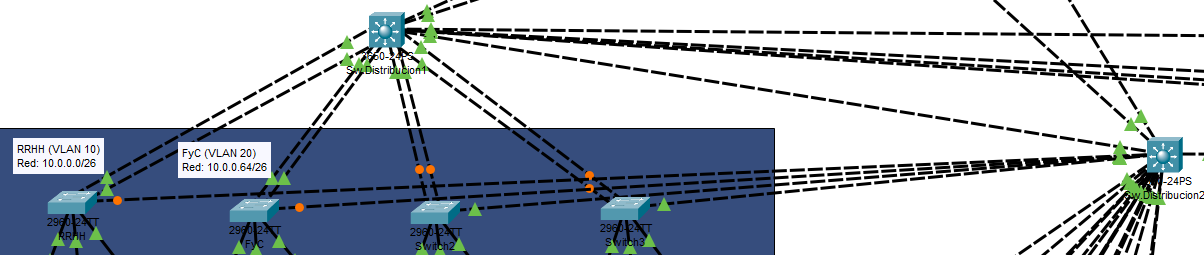
\includegraphics[width=0.6\textwidth]{Imágenes/hsrpSW.png}
    \caption{HSRP en Switches de Distribución en Hospital Son Espases}
    \label{fig:HSRPSW}
\end{figure}

También se ha configurado HSRP en los routers principales, permitiendo así que haya dos routers de repuesto por si el router principal falla y deja de dar servicio. En la Figura \ref{fig:HSRPRou} 
se pueden apreciar los tres routers redundantes.

\begin{figure}[H]
    \centering
    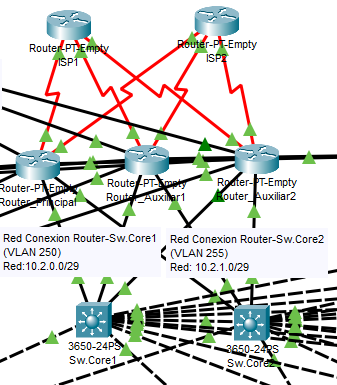
\includegraphics[width=0.5\textwidth]{Imágenes/HSRProut.png}
    \caption{HSRP en Routers en Hospital Son Espases}
    \label{fig:HSRPRou}
\end{figure}

\subsection{OSPF (Open Shortest Path First)}
Como protocolo de enrutamiento dinámico se ha implementado OSPF, detallado en la sección \ref{subsec:ospf}, 
tanto en la red del Hospital Son Espases como en la red de interconexión entre hospitales. 
\\ \\
En el caso de la red del Hospital Son Espases, se ha añadido una configuración extra, que permite definir el coste de las rutas OSPF, de esta forma se ha configurado la red de 
interconexión entre switches de distribución y switches core para que tengan un coste de 10, mientras que la red de interconexión de switches de distribución tengan un coste de 100. De
 esta forma forzamos a que las comunicaicones se hagan directamente entre los switches de distirbución y los switches core y que las conexiones entre los switches de distribución sean meramente redudnantes y que no 
congestionen la red innecesariamente.
\\ \\
El protocolo OSPF se ha configurado, en ambos diseños, en cada switch L3 y en los routers, ya que son los dispositivos de red que tienen capacidad de enrutamiento.

\subsection{EtherChannel}
Para aumentar el ancho de banda y proporcionar redundancia en los enlaces entre switches de distribución y switches de acceso, se ha configurado EtherChannel, detallado en la sección \ref{subsec:etherchannel}.
\\ \\
Como se ha comentado en la sección \ref{sec:criterios}, la redundancia a nivel de enlaces solo se ha configurado en la red del Hospital de Son Espases. A causa de las limitaciones de la herramienta Cisco Packet Tracer, referenciadas en la sección \ref{subsec:limites},
solo se ha podido implementar en algunas conexiones entre switches de acceso y switches de distribución, lo ideal sería implementarlo en tramos de mucho tráfico y en tramos donde hay una conexión entre elementos críticos, como por ejemplo la conexión entre los routers y los switches core.
\\ \\
En la Figura \ref{fig:EtherChannel} se muestra una conexión redundante a nivel de enlace en la red del Hospital Son Espases.

\begin{figure}[H]
    \centering
    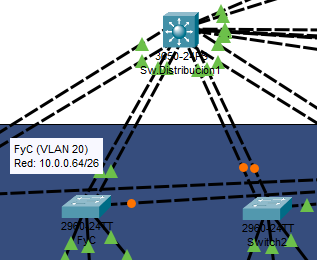
\includegraphics[width=0.5\textwidth]{Imágenes/Etherchannel.png}
    \caption{EtherChannel entre Switches de Acceso y Distribución en Hospital Son Espases}
    \label{fig:EtherChannel}
\end{figure}

\subsection{RSTP (Rapid Spanning-Tree Protocol)}


\section{Seguridad de la Red (cambiar)}
El diseño de la infraestructura de red hospitalaria simulada ha priorizado desde el inicio la seguridad como pilar esencial, dada la sensibilidad de los datos clínicos que se 
gestionan y la criticidad de los servicios asistenciales que dependen de ella. Además, la incorporación de dispositivos médicos conectados (IoMT) requieren unos controles de tráfico y 
acceso mas robustos.
\\ \\
En esta sección, se detallan las medidas de seguridad adopatadas en ambos diseños de red.
\subsection{ACLs}\label{subsec:acls}
Las ACLs permiten tener un control del tráfico que pasa por ciertos tramos, es por eso que, siguiendo con los requisitos establecidos en la sección \ref{subsec: TiposIoMT}, se han implementado las siguientes ACLs:
\begin{itemize}
    \item \textbf{En los routers:} 
    \begin{itemize}
        \item Permitir la conexión con Internet a los dispositivos de la red de invitados.
        \item Permitir la conexión desde Internet hasta el servidor web.
        \item Permitir paquetes DHCP, OSPF y HSRP.
        \item Denegar cualquier otro tipo de tráfico.
    \end{itemize}
    \item \textbf{Switch IoMT Planta 3:}
    \begin{itemize}
        \item Permitir la conexión de los dispositivos IoMT de tipo 1 con dispositivos de las áreas de servicios quirúrgicos, médicos y centrales.
        \item Permitir la conexión de los dispositivos IoMT de tipo 2 con dispositivos del departamento de la UCI.
        \item Permitir la conexión de los dispositivos IoMT de tipo 3 con el dispositivo autorizado de la UCI.
        \item Permitir paquetes DHCP y OSPF.
        \item Denegar cualquier otro tipo de tráfico.
    \end{itemize}
    \item \textbf{Switch IoMT Planta 0,1 y 2:}
    \begin{itemize}
        \item Permitir la conexión de los dispositivos IoMT de tipo 1 con dispositivos de las áreas de servicios quirúrgicos, médicos y centrales.
        \item Permitir paquetes DHCP y OSPF.
        \item Denegar cualquier otro tipo de tráfico.
    \end{itemize}
    \item \textbf{Switches de Distribución:}
    \begin{itemize}
        \item Denegar la salida de paquetes hacia las áreas de servicios quirúrgicos, médicos y centrales.
        \item Permitir cualquier otro tipo de tráfico.
    \end{itemize}
    \item \textbf{Routers de la red de interconexión:}
    \begin{itemize}
        \item Denegar la conexión entre los dispositivos no autorizados con el servidor de archivos.
        \item Denegar la conexión entre los dispositivos de otros hospitales con dispositivos del hospital.
        \item Permitir cualquier otro tipo de tráfico.
    \end{itemize}
\end{itemize}

\subsection{DHCP Snooping}
Para evitar ataques de DHCP Spoofing, se ha configurado DHCP Snooping en todos los switches de acceso que no tengan enlaces redundantes (EtherChannel), ya que la herramienta Cisco Packet Tracer no permite 
configurar DHCP Spoofing en enlaces redundantes. Con la configuración de este mecanismo de seguridad, conseguimos que los dispositivos finales solo acepten las direcciones IP dadas por los servidores DHCP autorizados, 
ya que el switch de acceso descarta cualquier oferta de dirección IP proveniente de un servidor DHCP no autorizado \cite{cisco_dhcp_snooping}.
\\ \\
También se ha configurado la opción de limitar la cantidad de paquetes DHCP enviados al servidor DHCP para evitar saturaciones.
\\ \\
Este mecanismo de seguridad solo está configurado en la red del Hospital de Son Espases.

\subsection{VPN IPSec}
Para proprocionar seguridad a las interconexiones entre los routers de cada hospital, se ha configurado una VPN IPsec, detallada en la sección \ref{subsec:ipsec}, en la que se encriptan y autentican todos los paquetes IP que se transmiten a través de esa conexión.
De esta forma conseguimos una gran capa de seguridad que nos garantiza la confidencialidad, integridad y autenticidad de los datos que viajan por esa red IP.
\\ \\
Este mecansimo de seguridad solo esta implementado en la red de interconexión entre hospitales, ya que la red del Hospital Son Espases no tiene conexiones entre routers de otros hospitales. 
Además cabe recordar que la comunicación entre hospitales solo se puede realizar entre el dispositivo autorizado de un hospital con el servidor de archivos de otro hospital.

\subsection{SSH}
Para la administración remota segura de los dispositivos de red (routers y switches), se ha habilitado SSH como protocolo seguro de gestión, en sustitución de protocolos inseguros como Telnet. 
Esta configuración se ha implementado en todos los dispositivos de red (switches L2, switches L3 y routers). 

\subsection{Configuración DMZ}\label{subsec:dmz}
Para que la DMZ sea una zona segura para los servidores, se han implementado una serie de mecanismos de seguridad:
\begin{itemize}
    \item \textbf{"switchport port-security maximum 1":} Limita el número máximo de direcciones MAC permitidas en el puerto a 1.
    \item \textbf{"switchport port-security mac-address sticky":} Activa el aprendizaje automático de direcciones MAC en modo "sticky", estas direcciones se almacenan en la configuración de ejecución, permitiendo que el puerto solo acepte dispositivos previamente conectados sin necesidad de configurar manualmente cada MAC.
    \item \textbf{"switchport port-security violation shutdown":} Deshabilita el puerto automáticamente cuando se detecta una violación de seguridad (por ejemplo, la conexión de un dispositivo con una MAC diferente a la permitida).
\end{itemize}

\section{Redes Completas}

Para ver las redes completas de la red del Hospital Son Espases y la red de interconexión entre hospitales, ver el anexo \ref{anexo:redcompletasonespas} y \ref{anexo:redcompletahosp}, respectivamente.

\subsection{Leyenda}
Como se puede apreciar en la Figura \ref{fig:SonEspases}, todas las areas estan coloreadas, esto es así para poder 
ubicarlas físicamente dentro del hospital, teniendo en cuenta lo mencionado en la sección \ref{subsubsec:dispsoicion}. 

\begin{itemize}
    \item \textbf{Rojo:} Área de Servicios Quirúrgicos.
    \item \textbf{Verde:} Área de Servicios Médicos.
    \item \textbf{Naranja:} Área de Servicios Centrales.
    \item \textbf{Azul:} Área de Administración.
    \item \textbf{Azul oscuro:} UCI.
    \item \textbf{Amarillo:} Área de Hospitalización.
    \item \textbf{Verde oscuro:} Área de Investigación.
    \item \textbf{Marrón:} Área de Atención al Paciente.
    \item \textbf{Rosa:} Área de Servidores y Dispositivos de Red.
    \item \textbf{Morado:} Área de Docencia.
\end{itemize}
